%
%   This program is free software: you can redistribute it and/or modify
%   it under the terms of the GNU General Public License as published by
%   the Free Software Foundation, either version 3 of the License, or
%   (at your option) any later version.
%
%   This program is distributed in the hope that it will be useful,
%   but WITHOUT ANY WARRANTY; without even the implied warranty of
%   MERCHANTABILITY or FITNESS FOR A PARTICULAR PURPOSE.  See the
%   GNU General Public License for more details.
%
%   You should have received a copy of the GNU General Public License
%   along with this program.  If not, see <http://www.gnu.org/licenses/>.
%

% Version: $Revision$

The Simple CLI provides full access to all Weka classes, i.e., classifiers, filters, clusterers, etc., but without the hassle of the CLASSPATH (it facilitates the one, with which Weka was started).

It offers a simple \textit{Weka shell} with separated commandline and output.

\begin{center}
	\epsfig{file=images/simplecli/simplecli_main.eps,height=10cm,angle=-90}
\end{center}


\section{Commands}
The following commands are available in the Simple CLI:
\begin{itemize}
	\item \texttt{java <classname> [<args>]} \\
		invokes a java class with the given arguments (if any)
	\item \texttt{break} \\
		stops the current thread, e.g., a running classifier, in a friendly manner
	\item \texttt{kill} \\
		stops the current thread in an unfriendly fashion
	\item \texttt{cls} \\
		clears the output area
	\item \texttt{capabilities <classname> [<args>]} \\
		lists the capabilities of the specified class, e.g., for a classifier
		with its options:
		{\small \begin{verbatim}
 		capabilities weka.classifiers.meta.Bagging -W weka.classifiers.trees.Id3
		\end{verbatim}}
	\item \texttt{exit} \\
		exits the Simple CLI
	\item \texttt{help [<command>]} \\
		provides an overview of the available commands if without a command name as argument, otherwise more help on the specified command
\end{itemize}


\section{Invocation}
In order to invoke a Weka class, one has only to prefix the class with "java". This command tells the Simple CLI to load a class and execute it with any given parameters. E.g., the J48 classifier can be invoked on the iris dataset with the following command:
\begin{verbatim}
	java weka.classifiers.trees.J48 -t c:/temp/iris.arff
\end{verbatim}

This results in the following output: 
\begin{center}
	\epsfig{file=images/simplecli/simplecli_j48.eps,height=7cm,angle=-90}
\end{center}


\section{Command redirection}
Starting with this version of Weka one can perform a basic redirection:

\begin{verbatim}
	java weka.classifiers.trees.J48 -t test.arff > j48.txt
\end{verbatim}

\noindent \textbf{Note:} the \texttt{>} must be preceded and followed by a space, otherwise it is not recognized as redirection, but part of another parameter.

\section{Command completion}
Commands starting with java support completion for classnames and filenames via Tab (\texttt{Alt+BackSpace} deletes parts of the command again). In case that there are several matches, Weka lists all possible matches.

\begin{itemize}
	\item \textbf{package name completion}
		\begin{verbatim}
			java weka.cl<Tab>
		\end{verbatim}
		results in the following output of possible matches of package names:
		\begin{verbatim}
			Possible matches:
			  weka.classifiers
			  weka.clusterers
		\end{verbatim}
	\item \textbf{classname completion}
		\begin{verbatim}
			java weka.classifiers.meta.A<Tab>
		\end{verbatim}
		lists the following classes
		\begin{verbatim}
		Possible matches:
		  weka.classifiers.meta.AdaBoostM1
		  weka.classifiers.meta.AdditiveRegression
		  weka.classifiers.meta.AttributeSelectedClassifier
		\end{verbatim}
	\item \textbf{filename completion} \\
	      In order for Weka to determine whether a the string under the cursor is a classname or a filename, filenames need to be absolute (Unix/Linx: \texttt{/some/path/file}; Windows: C:$\backslash$Some$\backslash$Path$\backslash$file) or relative and starting with a dot (Unix/Linux: \texttt{./some/other/path/file}; Windows: .$\backslash$Some$\backslash$Other$\backslash$Path$\backslash$file).
\end{itemize}

